\documentclass[12pt]{article}

\usepackage{amsmath}
\usepackage{amssymb}
\usepackage{graphicx}
\graphicspath{{figures/}}
\usepackage{hyperref}
\usepackage[margin=1in]{geometry}
\usepackage{natbib}
\bibliographystyle{aasjournal}

\title{Real-Space versus Fourier-Space Sampling of Initial Conditions\\
for Cosmological $N$-body Simulations}
\author{Notes based on \citet{Pen1997}, \citet{Sirko2005}, and \citet{Hahn2011}}
\date{\today}

\begin{document}

\maketitle
\tableofcontents
\newpage

%----------------------------------------------------------------------
\section{Introduction}

Generating accurate initial conditions (ICs) for cosmological $N$-body
simulations requires populating a finite periodic box with a Gaussian
random density field whose statistical properties match those predicted
by linear perturbation theory. The standard procedure --- sampling the
matter power spectrum $P(k)$ at discrete Fourier modes --- has been used
since the earliest large-scale structure simulations. However, a series
of papers by \citet{Pen1997}, \citet{Sirko2005}, and \citet{Hahn2011}
demonstrated that this conventional ``$P$-sampled'' approach introduces
systematic errors in the real-space statistical properties of the
resulting field, particularly for small simulation volumes. These errors
arise from the way discrete Fourier sampling handles (or fails to handle)
long-wavelength modes near and beyond the box scale.

These notes summarise the key findings of all three papers, describe the
proposed remedies, and discuss the implications for modern IC generators
such as \textsc{music2} \citep{Hahn2011} and
\textsc{monofonIC}\footnote{\url{https://github.com/ohahn/monofonic}},
both of which continue to use $k$-space sampling for uniform-grid ICs.

%----------------------------------------------------------------------
\section{The Conventional ($P$-sampled) Method}
\label{sec:conventional}

\subsection{Algorithm}

In the conventional approach the density field $\delta(\mathbf{x})$ is
generated by the following steps:
%
\begin{enumerate}
  \item Draw a complex Gaussian random field $\tilde{\mu}(\mathbf{k})$
        with zero mean and unit variance for each mode on a
        three-dimensional grid of spacing $\Delta k = 2\pi/L$.
  \item Multiply each mode by the square root of the desired power
        spectrum,
        \begin{equation}
          \tilde{\delta}(\mathbf{k}) = \sqrt{P(\|\mathbf{k}\|)}\;
          \tilde{\mu}(\mathbf{k}),
          \label{eq:kspace}
        \end{equation}
        where $P(k) \equiv \alpha\,k^{n_s}\,\mathcal{T}^2(k)$, with
        $\mathcal{T}(k)$ the matter transfer function, $n_s$ the
        primordial spectral index, and $\alpha$ a normalisation constant.
  \item Inverse-Fourier-transform to obtain the real-space overdensity
        $\delta(\mathbf{x})$.
\end{enumerate}
%
The displacement and velocity fields are then obtained from $\delta$ via
Lagrangian perturbation theory (LPT), solving Poisson's equation for the
gravitational potential.

\subsection{Equivalence to Real-Space Convolution}

As noted by \citet{Pen1997} and \citet{Hahn2011}, equation~\eqref{eq:kspace}
is equivalent to a convolution in real space,
\begin{equation}
  \delta(\mathbf{x}) = \mathcal{T}(\|\mathbf{x}\|) \star \mu(\mathbf{x}),
  \label{eq:realconv}
\end{equation}
where $\mathcal{T}(r)$ is the Fourier transform of
$\tilde{\mathcal{T}}(k) \equiv \alpha^{1/2}\,k^{n_s/2}\,\mathcal{T}(k)$
and $\star$ denotes convolution. For an \emph{infinite} periodic volume
the two procedures are mathematically identical by the convolution
theorem. The differences arise only when the volume is finite.

%----------------------------------------------------------------------
\section{The Truncation Error: Lost Long-Wavelength Power}
\label{sec:truncation}

\subsection{Discrete Fourier Sampling and Sparse Modes}

On a finite periodic grid of side $L$, the allowed wavenumbers are
$\mathbf{k} = (i,j,k)\,\Delta k$ with $\Delta k = 2\pi/L$.  The $k$-space
approach evaluates $P(k)$ \emph{exactly} at these discrete values and
sets all other modes --- in particular all modes with
$|\mathbf{k}| < \Delta k$, i.e.\ super-box modes --- to zero.

Two distinct but related problems arise from this discrete sampling.

\textbf{(1) The $k=0$ mode is forced to zero.}
The mode $\tilde{\delta}(\mathbf{0})$ is drawn from a Gaussian with
variance $P(k=0)$.  For standard CDM-like power spectra,
\begin{equation}
  P(k) \propto k^{n_s} \xrightarrow{k \to 0} 0,
\end{equation}
so $P(k=0) = 0$ exactly%
\footnote{The scaling $P(k) \propto k^{n_s}$ at small $k$ follows from
  the primordial Harrison--Zel'dovich--Peebles spectrum generated by
  inflation.  Inflation produces nearly scale-invariant curvature
  perturbations $\mathcal{P}_\mathcal{R}(k) \propto k^{n_s-1}$ with
  $n_s \approx 0.96$ (Planck 2018).  Converting to the matter
  overdensity via Poisson's equation ($\nabla^2\Phi \propto \delta$,
  introducing $k^2$) and the Bardeen relation ($\Phi \propto
  \mathcal{R}/k^2$ on super-horizon scales, introducing another
  $k^{-2}$) gives $P_\delta(k) \propto k^{n_s}\,T^2(k)$, where the
  transfer function $T(k) \to 1$ as $k \to 0$.  Since $n_s > 0$,
  $P(k) \to 0$ as $k \to 0$.  Physically, $k = 0$ would correspond to
  a perfectly uniform density perturbation across the entire universe,
  which is forbidden by energy conservation.} and $\tilde{\delta}(\mathbf{0}) = 0$ with
probability one in every realisation.  This is \emph{not} a consequence
of the Dirac comb; it is simply because the analytic power spectrum
vanishes at $k=0$.  The physical meaning is that the mean overdensity
of the simulation box is constrained to be exactly zero,
\begin{equation}
  \bar{\delta}_\mathrm{box} \equiv 0
  \quad \Longleftrightarrow \quad
  \int \xi(\mathbf{x})\,d^3x = 0,
  \label{eq:zeromean}
\end{equation}
whereas in reality the mean overdensity of a randomly placed finite
volume is drawn from a nonzero distribution.

\textbf{(2) Long-wavelength power between grid points is missed.}
Discrete sampling evaluates $P$ at exactly the grid frequencies and
ignores the power that lies \emph{between} them.  This is where the
Dirac comb picture is relevant: sampling $P(k)$ at $\mathbf{k}_n =
n\,\Delta k$ is equivalent to multiplying the continuous spectrum by
$\mathrm{III}_{\Delta k}(k)$, which in real space convolves $\xi(r)$
with a periodic image sum.  Near $k = 0$, where $P(k)$ rises steeply
from zero, even a spacing of $\Delta k = 2\pi/L$ represents a
significant ``bin width'' over which the power is not captured.  The
correct effective power at $k = 0$ should be an average of $P(k')$
over the bin width:
\begin{equation}
  P^\mathrm{grid}(0) = \int P(|\mathbf{k}'|)\,W_C(\mathbf{k}')\,d^3k'
  \;\neq\; 0,
  \label{eq:pgrid0}
\end{equation}
where $\tilde{W}_C(\mathbf{k})$ is the Fourier transform of the box
window function, described in detail below.  The $P$-sampled approach
replaces this integral with the single value $P(0) = 0$, losing all
the power from neighbouring modes.

Both effects share the same remedy: the convolution picture of
\citet{Pen1997}, described in Section~\ref{sec:convolution}.

\subsubsection*{The box window function $W_C$}

In real space, $W_C(\mathbf{x})$ is the indicator function of the
simulation volume --- a three-dimensional cubical top-hat of side $L$:
\begin{equation}
  W_C(\mathbf{x}) = \begin{cases}
    1 & |x_i| \leq L/2 \text{ for all } i = 1,2,3, \\
    0 & \text{otherwise.}
  \end{cases}
\end{equation}
Its Fourier transform factors into a product of sinc functions along
each Cartesian axis,
\begin{equation}
  \tilde{W}_C(\mathbf{k})
  = \int W_C(\mathbf{x})\,e^{-i\mathbf{k}\cdot\mathbf{x}}\,d^3x
  = L^3 \prod_{i=1}^{3} \mathrm{sinc}\!\left(\frac{k_i L}{2}\right),
  \qquad \mathrm{sinc}(x) \equiv \frac{\sin x}{x},
  \label{eq:WC}
\end{equation}
where the product reflects the separability of the cubical geometry.
The characteristic width of each sinc factor in $k$-space is
$\sim 2\pi/L = \Delta k$, one fundamental mode spacing.  The function
is plotted in Figure~\ref{fig:boxwindow}.

\begin{figure}[t]
  \centering
  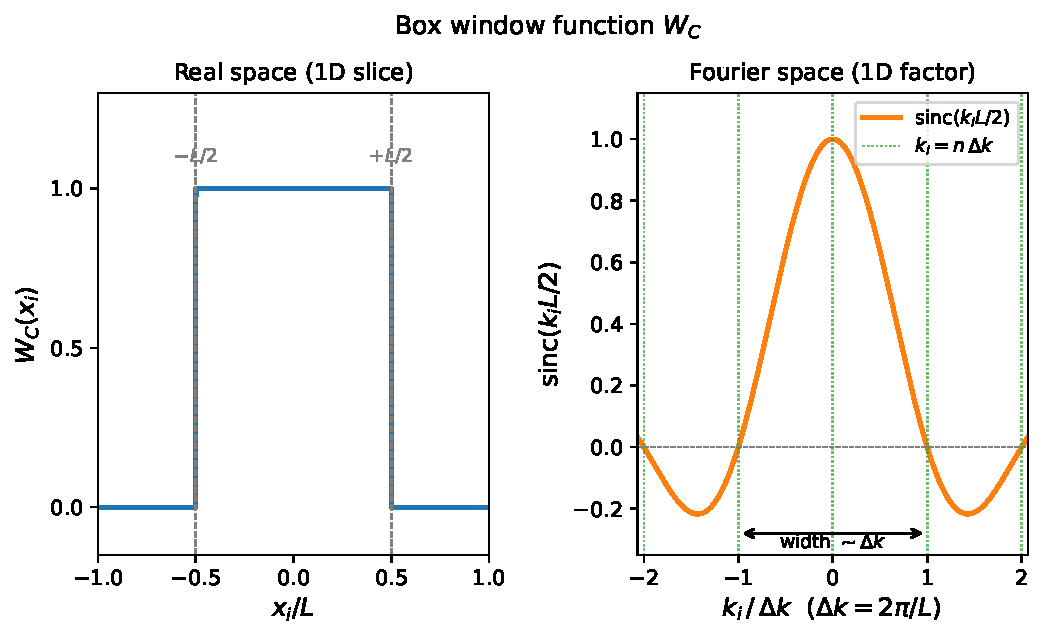
\includegraphics[width=0.85\textwidth]{box_window.pdf}
  \caption{The box window function $W_C$ in real space (left, 1D
    slice) and Fourier space (right, one sinc factor).  In real space
    it is a cubical top-hat of side $L$.  In Fourier space each
    Cartesian factor is $\mathrm{sinc}(k_i L/2)$, with width
    $\sim\Delta k = 2\pi/L$ (indicated by the double arrow).  The
    dotted vertical lines mark the discrete grid frequencies
    $k_i = n\,\Delta k$.  The sinc is unity at $k_i = 0$ and zero at
    $k_i = \pm 2\Delta k, \pm 4\Delta k, \ldots$, so it smoothly
    averages $P(k)$ over a bin of width $\sim\Delta k$ around each
    grid point.}
  \label{fig:boxwindow}
\end{figure}

The role of $\tilde{W}_C$ in equation~\eqref{eq:pgrid0} is to perform
exactly this bin-averaging.  Physically, restricting the density field
to the simulation box (multiplication by $W_C(\mathbf{x})$ in real
space) is equivalent to convolving its power spectrum with
$\tilde{W}_C(\mathbf{k})$ in Fourier space.  At $k = 0$, instead of
evaluating $P(0) = 0$, the convolution integrates $P(k')$ over a shell
of width $\sim\Delta k$:
\begin{equation}
  P^\mathrm{grid}(0)
  = \int P(|\mathbf{k}'|)\,\tilde{W}_C(\mathbf{k}')\,d^3k'
  \approx 4\pi \int_0^{\Delta k} P(k')\,k'^2\,dk'
  > 0.
\end{equation}
This is precisely the variance of the simulation volume that the
$P$-sampled approach misses by evaluating $P$ at $k = 0$ directly.

\subsection{Effect on $\sigma_8$ and the Correlation Function}

\begin{figure}[t]
  \centering
  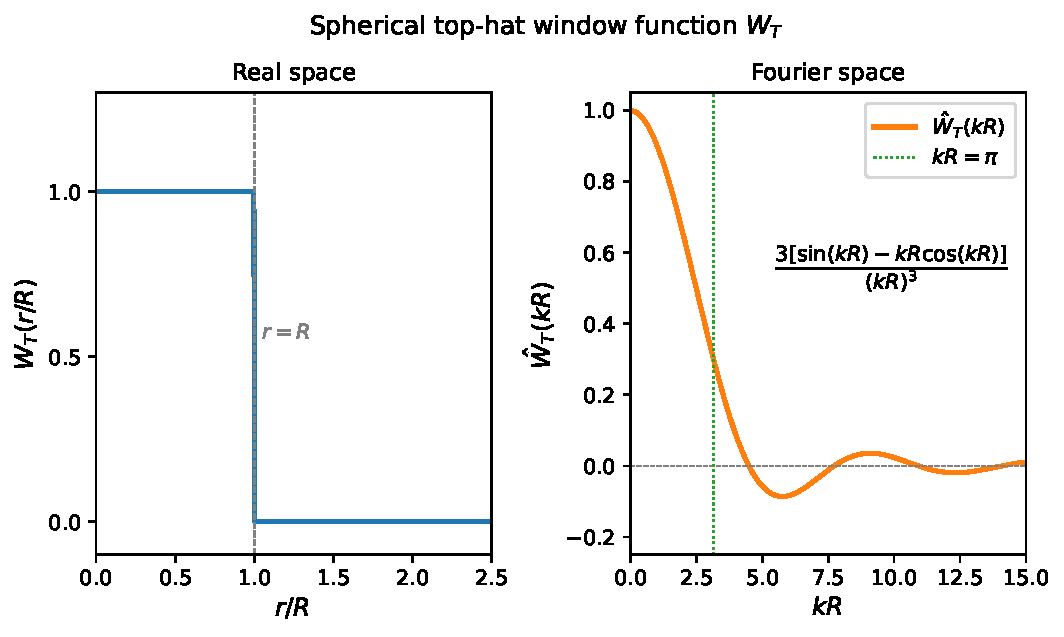
\includegraphics[width=0.85\textwidth]{tophat_window.pdf}
  \caption{The spherical top-hat window function $W_T$ in real space
    (left) and Fourier space (right).  In real space it is a step
    function of radius $R$.  Its Fourier transform
    $\hat{W}_T(kR) = 3[\sin(kR) - kR\cos(kR)]/(kR)^3$ weights modes
    in the mass-variance integral $\sigma_R^2 =
    (2\pi^2)^{-1}\int P(k)\,\hat{W}_T^2(kR)\,k^2\,dk$.  Because
    $\hat{W}_T(kR) \approx 1$ for $kR \ll 1$, long-wavelength modes
    ($k \lesssim 1/R$) contribute significantly to $\sigma_R^2$; their
    absence in $P$-sampled ICs with box size $L \sim R$ directly
    suppresses the measured variance.}
  \label{fig:tophat}
\end{figure}

\citet{Gelb1994} first quantified the consequence: for a box of side
$L = 51.2\,h^{-1}$\,Mpc the rms mass fluctuation on $8\,h^{-1}$\,Mpc
spheres, $\sigma_8$, was found to be \emph{systematically 40\% lower}
than the analytical value.  \citet{Pen1997} identified the physical
cause: for CDM power spectra with slope $n \to -3$ on small scales,
most of the variance on small top-hat spheres receives contributions from
modes with $k \lesssim 2\pi/L$ that are simply absent from the box.
Truncation in Fourier space therefore underestimates $\sigma_8$.

The underestimate can be understood from the expression for the top-hat
variance,
\begin{equation}
  \sigma_R^2 = \frac{1}{2\pi^2}\int_0^\infty P(k)\,\hat{W}_T^2(kR)\,k^2\,dk,
\end{equation}
where $\hat{W}_T(kR) = 3[\sin(kR) - kR\cos(kR)]/(kR)^3$ is the
top-hat window.  The lower limit of the integral is effectively replaced
by $2\pi/L$, cutting off the contribution of long waves.

Similarly, \citet{Sirko2005} showed using Figure~1 of that paper that the
correlation function $\xi(r)$ computed from $P$-sampled ICs in boxes of
$L = (100, 200, 400, 800)\,h^{-1}$\,Mpc systematically falls below the
true (infinite-volume) value at large $r$, with the discrepancy growing
as $L$ decreases.  \citet{Hahn2011} show (their Figure~2) that the
$k$-space sampled correlation function even shows a \emph{stronger drop}
at large $r$ compared to the periodic real-space kernel, attributing this
to an integral constraint:
\begin{equation}
  0 = \int_\mathcal{D} \xi(\mathbf{x})\,d^3x
    \simeq 4\pi \int_0^{L/2} \xi(r)\,r^2\,dr,
  \label{eq:integralconstraint}
\end{equation}
which follows directly from equation~\eqref{eq:zeromean}.  This constraint
forces an additive negative offset on $\xi(r)$, suppressing it at large
separations.

\subsection{The DC Mode Variance}
\label{sec:dcmode}

\citet{Sirko2005} isolated the dominant source of the $\sigma_8$ bias as
the \emph{missing DC mode variance}.  In the real universe a randomly
placed box of side $L$ has a mean overdensity $\Delta_0$ drawn from a
Gaussian distribution of variance $P_L(0)/V$, where
$P_L(0) \equiv \int_0^{L/2} 4\pi\xi(r)\,r^2\,dr$ is the
box-convolved power at $k=0$ and $V = L^3$ is the box volume.  The
contribution of this DC mode to $\sigma_8^2$ is
\begin{equation}
  \sigma_{8,\mathrm{DC}}^2 = P_L(0)/V,
\end{equation}
which is $\sim 6\%$ of $\sigma_{8,\mathrm{theory}}^2$ for
$L = 50\,h^{-1}$\,Mpc.  Because the $P$-sampled approach fixes
$\Delta_0 = 0$ in every realisation, this variance is entirely absent.

Furthermore, the \emph{variance of the DC mode} across an ensemble of
realisations is suppressed: for $L = 50\,h^{-1}$\,Mpc the characteristic
overdensity $\Delta_0$ can be as large as 30\% of the rms, so individual
realisations differ markedly in their large-scale gravitational
environment.  Setting $\Delta_0 = 0$ artificially removes this
box-to-box scatter, which affects the nonlinear growth of structure and
the abundance of massive haloes.

%----------------------------------------------------------------------
\section{The Convolution ($\xi$-sampled) Approach}
\label{sec:convolution}

\subsection{The Pen (1997) Convolution Picture}

\citet{Pen1997} proposed to impose periodicity on the \emph{real-space
correlator} rather than on the power spectrum.  The algorithm is:
%
\begin{enumerate}
  \item Generate a white-noise field $\mu(\mathbf{x})$ (zero mean, unit
        variance) on the grid.
  \item Define the \emph{correlation kernel} $W_r(\mathbf{x})$ as the
        inverse Fourier transform of $[P(k)]^{1/2}$:
        \begin{equation}
          \tilde{W}_r(\mathbf{k}) = [P(|\mathbf{k}|)]^{1/2}
          \quad \Longleftrightarrow \quad
          W_r(\mathbf{x}) = \int \frac{d^3k}{(2\pi)^3}\,
          [P(|\mathbf{k}|)]^{1/2}\,e^{i\mathbf{k}\cdot\mathbf{x}}.
          \label{eq:corrkernel}
        \end{equation}
        The name ``correlation kernel'' comes from the fact that its
        autocorrelation reproduces the two-point correlation function,
        $\xi(r) = \langle W_r(\mathbf{x})\,W_r(\mathbf{x}+\mathbf{r})\rangle$,
        which follows from the Wiener--Khinchin theorem since
        $|\tilde{W}_r(\mathbf{k})|^2 = P(k)$.
  \item Convolve: $\delta(\mathbf{x}) = \int \mu(\mathbf{x}')\,
        W_r(\mathbf{x}-\mathbf{x}')\,d^3x'$,
        computed efficiently via FFT.  In Fourier space this is simply
        $\tilde{\delta}(\mathbf{k}) = [P(k)]^{1/2}\,\tilde{\mu}(\mathbf{k})$,
        identical to the conventional approach for an infinite volume.
        The difference arises on a finite periodic grid, where Pen
        imposes periodicity on $\xi(r)$ (and hence on $W_r$) rather
        than on $P(k)$ directly.
\end{enumerate}
%
In Fourier space this convolution is equivalent to replacing the power
spectrum with the \emph{windowed} (or convolved) power spectrum:
\begin{equation}
  P^\mathrm{grid}(\mathbf{k}) = \int P(|\mathbf{k}'|)\,
  W_C(\mathbf{k}'-\mathbf{k})\,d^3k',
  \label{eq:pgrid}
\end{equation}
where $W_C(\mathbf{k})$ is the Fourier transform of the cubical box
window function.  The effect of this convolution is most pronounced at
small $k$: at $k=0$, where the analytic $P(k\to 0) \to 0$ for scale-
invariant spectra, the windowed version takes a finite value equal to
the variance of the simulation volume.  This is precisely the power that
the $P$-sampled approach loses.

Figure~\ref{fig:pgrid} illustrates $P^\mathrm{grid}(k)$ computed from
the CLASS matter power spectrum at $z=45$ for three box sizes, using
the spherical approximation (truncating $\xi(r)$ at $r = L/2$).  At
large $k$ the windowed spectrum converges to $P(k)$ because the
contribution of modes beyond the truncation radius is negligible.  At
small $k$ near the fundamental mode $k_f = 2\pi/L$ (vertical dotted
lines), $P^\mathrm{grid}(k)$ exceeds $P(k)$ significantly, with the
excess growing as $L$ decreases.  The ratio panel quantifies this: for
$L = 25\,h^{-1}$\,Mpc the windowed power near $k_f$ is several times
larger than the raw $P(k)$, reflecting the substantial contribution
of super-box modes to the variance on those scales.

\begin{figure}[t]
  \centering
  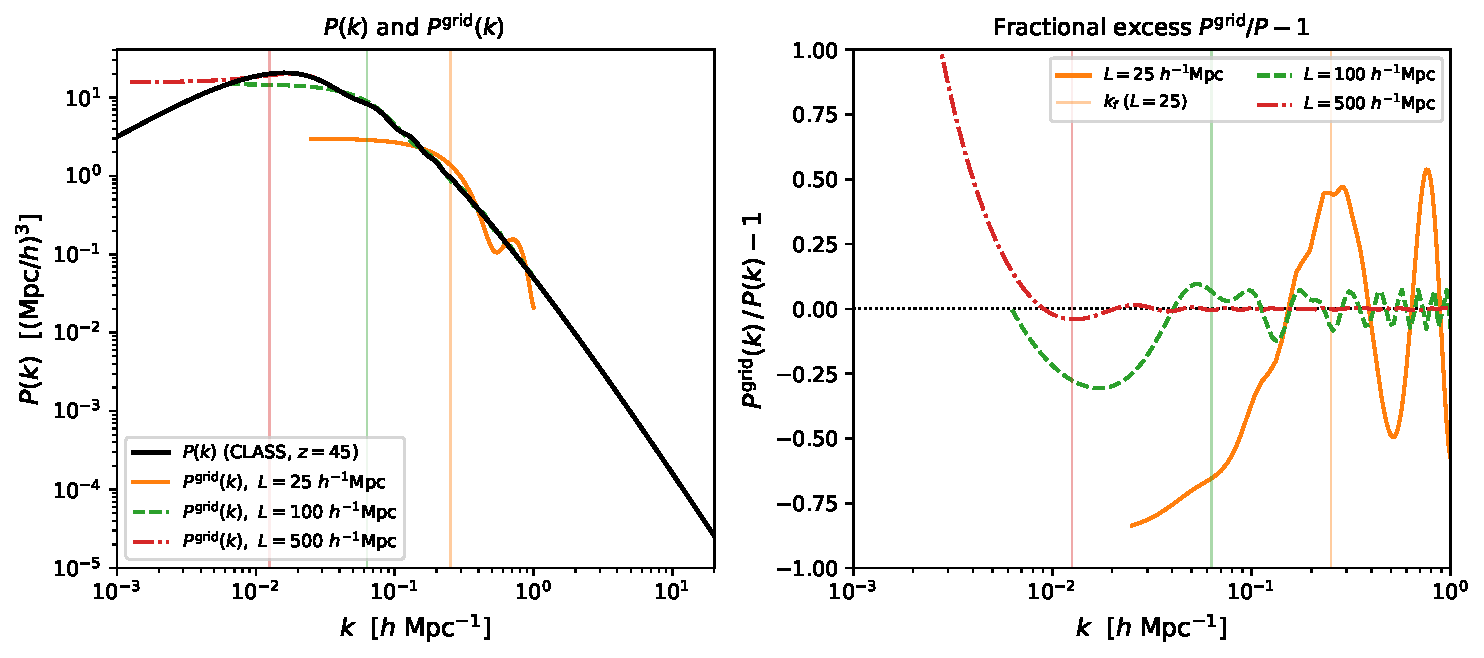
\includegraphics[width=\textwidth]{pgrid_comparison.pdf}
  \caption{\textit{Left:} The CLASS matter power spectrum $P(k)$ at
    $z=45$ (black) compared with the windowed power spectrum
    $P^\mathrm{grid}(k)$ (eq.~\ref{eq:pgrid}) for three box sizes
    $L = 25$, 100, and $500\,h^{-1}$\,Mpc.  Vertical dotted lines
    mark the fundamental mode $k_f = 2\pi/L$ for each box.
    $P^\mathrm{grid}(k)$ is computed by Hankel-transforming $P(k)$ to
    $\xi(r)$, truncating at $r = L/2$, and transforming back.
    \textit{Right:} Ratio $P^\mathrm{grid}(k)/P(k)$.  The ratio
    exceeds unity near $k_f$ and approaches unity at large $k$,
    with the excess growing for smaller boxes.  The $P$-sampled
    approach uses $P(k)$ directly, missing the excess power near
    $k_f$ and setting it to zero at $k=0$.}
  \label{fig:pgrid}
\end{figure}

\citet{Pen1997} showed (his Figure~1) that the convolution picture
recovers the correct $\sigma_8$ for box sizes $L \gtrsim 32\,h^{-1}$\,Mpc,
while the standard $k$-space approach requires $L \gtrsim 100\,h^{-1}$\,Mpc
to achieve 10\% accuracy.  The convolution picture produces exact
correlation functions for $r < L/2$ and exact top-hat variances for
$R \leq L/4$.

\subsection{The Sirko (2005) Implementation}

\citet{Sirko2005} described the $\xi$-sampled approach as convolving
$P(k)$ with the box window function \emph{before} discrete sampling.
Specifically, one computes the correlation function $\xi(r)$ by inverse
Fourier transforming $P(k)$, sets $\xi(r) = 0$ for $|r_i| > L/2$
(Cartesian truncation at the box boundary), and then Fourier transforms
back to obtain $P_L(k)$.  This $P_L(k)$ is then sampled at the discrete
grid modes.  The crucial step is that $P_L(k=0) \neq 0$, so the DC
mode receives a proper nonzero draw from the Gaussian distribution of
variance $P_L(0)/V$.

Using an ensemble of 100 realisations for $L = 50\,h^{-1}$\,Mpc,
$N = 32^3$, \citet{Sirko2005} demonstrated:
%
\begin{itemize}
  \item The \emph{ensemble mean} $\sigma_8$ of $P$-sampled ICs is
        $\sim 6\%$ below the theoretical value; $\xi$-sampled ICs
        correct this bias.
  \item The \emph{ensemble variance} of $\sigma_8$ is also reduced in
        $P$-sampled ICs because the DC mode is frozen; $\xi$-sampled
        ICs restore the correct box-to-box scatter.
  \item The correlation function $\xi(r)$ from $P$-sampled ICs shows a
        large systematic offset below the theory curve for $r \gtrsim
        20\,h^{-1}$\,Mpc (his Figure~9), while $\xi$-sampled ICs agree
        with theory within statistical scatter.
  \item The power spectrum $P(k)$ looks nearly identical between the two
        methods (his Figure~10) --- the difference is \emph{invisible in
        Fourier space} and only appears in real-space statistics.
\end{itemize}

\subsection{Hahn \& Abel (2011): Real-Space Kernel for Multi-Scale ICs}

\citet{Hahn2011} recast the convolution picture in terms of a real-space
transfer function kernel $\mathcal{T}_\mathcal{R}(r)$, defined as the
Fourier transform of the $k$-space transfer function $\tilde{\mathcal{T}}(k)$
computed using the \textsc{fftlog} algorithm \citep{Talman1978,
Hamilton2000}:
\begin{equation}
  \mathcal{T}_\mathcal{R}(r) = \frac{1}{(2\pi)^3}
  \int_\mathbb{R} \tilde{\mathcal{T}}(\mathbf{k})\,
  e^{i\mathbf{x}\cdot\mathbf{k}}\,d^3k
  = \frac{4\pi}{(2\pi)^3}\int_0^\infty
  \tilde{\mathcal{T}}(k)\,\frac{\sin(kr)}{kr}\,k^2\,dk.
  \label{eq:realkernel}
\end{equation}
The density field is then obtained by convolving this kernel with the
white-noise field $\mu(\mathbf{x})$ on the simulation grid,
\begin{equation}
  \delta(\mathbf{x}_{ijk}) = \mathcal{T}_\mathcal{R}(\|\mathbf{x}_{ijk}\|)
  \star \mu(\mathbf{x}_{ijk}),
\end{equation}
implemented via FFT on a periodic grid.

The primary motivation for \citet{Hahn2011} to adopt the real-space
kernel was the multi-scale nested grid structure required for zoom
simulations.  In a zoom setup, the refinement region has much higher
resolution than the surrounding volume, separated by coarse-fine
boundaries.  A global FFT over all levels is infeasible, but the
real-space kernel $\mathcal{T}_\mathcal{R}(r)$ decays with $r$ and can
be applied locally, properly coupling long-wavelength modes from the
coarse grid to the fine-grid density field across boundaries.

An additional advantage noted by \citet{Hahn2011} is that the
non-periodic real-space kernel does not impose the zero-mean constraint
of equation~\eqref{eq:integralconstraint}, so the correlation function
$\xi(r)$ is reproduced correctly at large $r$ without the systematic
suppression seen in the $k$-space approach.

%----------------------------------------------------------------------
\section{Symmetric Advantages and Disadvantages}
\label{sec:comparison}

The two approaches err in \emph{opposite} directions, as noted by
\citet{Pen1997}:
%
\begin{itemize}
  \item \textbf{$P$-sampled (k-space):} Underestimates $\sigma_8$ and
        $\xi(r)$ at large $r$ because long-wavelength modes are lost.
        The DC mode is frozen to zero, removing box-to-box variance.
  \item \textbf{$\xi$-sampled (real-space):} Slightly overestimates
        $\sigma_8$ because periodicity causes the forced-periodic
        correlator to increase beyond the periodicity radius $r = L/2$
        rather than decaying, inflating $\sigma_R^2$ for $R \gtrsim L/4$.
        \citet{Pen1997} shows this overestimate is typically $\lesssim
        10\%$ and is much smaller than the underestimate of the $P$-sampled
        approach.
\end{itemize}

For uniform periodic boxes, the two methods are \emph{mathematically
equivalent} in the limit $L \to \infty$.  The practical rule of thumb
from \citet{Pen1997} is that a box is ``small'' --- i.e.\ the truncation
error is non-negligible --- when the variance on the box scale exceeds
10\%, which for standard CDM cosmologies corresponds to $L \lesssim 50\,
h^{-1}$\,Mpc.

%----------------------------------------------------------------------
\section{A Note on Poisson Noise Subtraction}
\label{sec:shotnoise}

\citet{Sirko2005} includes an important warning (his \S10) about
subtracting Poisson shot noise from measured power spectra of IC
particle distributions.  The conventional justification is that
discreteness introduces a delta-function contribution to the correlation
function of amplitude $1/\bar{n}$ (where $\bar{n}$ is the mean particle
number density), which adds a white noise floor $P_\mathrm{shot} = V/N$
to the measured $P(k)$.

However, \citet{Sirko2005} argues that ICs generated from a lattice (or
glass) are \emph{not} a Poisson distribution.  The lattice has zero
power at $k = 0$, so there is no initial power at sub-Nyquist scales
that would justify a Poisson subtraction.  The spikes visible at high
$k$ in early-time power spectra (his Figure~10, $a = 0.001$) are
\emph{Bragg peaks} from the crystal-like lattice, not Poisson noise.
These wash out by $a \sim 0.2$ as the lattice structure is erased by
gravitational evolution.

The conclusion is that \textbf{subtracting $V/N$ from the measured
$P(k)$ of IC particle distributions is not justified} and can mask the
true discreteness structure, which is correlated (lattice-like) rather
than Poisson.

%----------------------------------------------------------------------
\section{Implications for Modern IC Generators}
\label{sec:modern}

Both \textsc{music2} \citep{Hahn2011} and \textsc{monofonIC} apply the
transfer function in Fourier space for uniform-grid runs.  The core
operation in \textsc{monofonIC} (\texttt{src/ic\_generator.cc}) is:
%
\begin{verbatim}
  delta = wn * the_cosmo_calc->get_amplitude(kmod, delta_matter);
\end{verbatim}
%
where \texttt{get\_amplitude} returns
$A(k) = k^{n_s/2}\,\mathcal{T}(k)\,\sqrt{P_\mathrm{norm}}$.
This is a pointwise multiplication of the white-noise Fourier modes
$\tilde{\mu}(\mathbf{k})$ by $\tilde{\mathcal{T}}(k)$ --- precisely the
$P$-sampled approach of equation~\eqref{eq:kspace}.

This means both codes carry the following biases for small or
moderate-sized boxes:
%
\begin{enumerate}
  \item $\sigma_8$ is systematically underestimated by $\sim 6\%$
        ($\sim 40\%$) for $L = 50$ ($L \sim 10$)\,$h^{-1}$\,Mpc.
  \item The DC mode is frozen to zero; ensemble statistics of $\sigma_8$
        and the correlation function are biased.
  \item $\xi(r)$ is suppressed at large $r$ relative to theory due to
        the integral constraint of equation~\eqref{eq:integralconstraint}.
\end{enumerate}
%
For large boxes ($L \gtrsim 100\,h^{-1}$\,Mpc) these effects are
negligible and $k$-space sampling is an excellent approximation.  For
zoom simulations, \textsc{music2} does employ the real-space kernel
approach to handle coarse-fine boundaries, recovering the advantages
described in \S\ref{sec:convolution}.

%----------------------------------------------------------------------
\section{Summary}

Table~\ref{tab:summary} summarises the key properties of the two
approaches.

\begin{table}[h]
\centering
\caption{Comparison of $P$-sampled and $\xi$-sampled IC generation.}
\label{tab:summary}
\begin{tabular}{lll}
\hline\hline
Property & $P$-sampled (k-space) & $\xi$-sampled (real-space) \\
\hline
DC mode & forced to zero & drawn from $\mathcal{N}(0,\,P_L(0)/V)$ \\
$\sigma_8$ bias & underestimate ($\sim$6\% at $L=50$) & slight overestimate ($\lesssim$10\%) \\
$\xi(r)$ at large $r$ & suppressed (integral constraint) & exact for $r < L/2$ \\
Box-to-box variance & underestimated & correct \\
$P(k)$ difference & negligible & negligible \\
Multi-scale zoom & requires global FFT & natural (local kernel) \\
Validity & $L \gtrsim 100\,h^{-1}$\,Mpc & $L \gtrsim 32\,h^{-1}$\,Mpc \\
\hline
\end{tabular}
\end{table}

The key insight from all three papers is that the real-space and
Fourier-space approaches differ only in how they handle the finite box
volume.  The $P$-sampled method treats the box as if it were a periodic
tiling of itself with exactly zero mean overdensity, while the
$\xi$-sampled method allows the box to be a random draw from the
universe with the correct distribution of mean densities.  The difference
is invisible in the power spectrum but significant in real-space
statistics --- particularly the two-point correlation function, mass
variance in spheres, and the distribution of massive haloes --- for
boxes smaller than $\sim 50\,h^{-1}$\,Mpc.

\bigskip
\begin{thebibliography}{99}
\bibitem[Gelb \& Bertschinger(1994)]{Gelb1994}
Gelb, J.~M.\ \& Bertschinger, E.\ 1994, \textit{ApJ}, 436, 491

\bibitem[Hahn \& Abel(2011)]{Hahn2011}
Hahn, O.\ \& Abel, T.\ 2011, \textit{MNRAS}, 415, 2101

\bibitem[Hamilton(2000)]{Hamilton2000}
Hamilton, A.~J.~S.\ 2000, \textit{MNRAS}, 312, 257

\bibitem[Pen(1997)]{Pen1997}
Pen, U.-L.\ 1997, \textit{ApJ}, 490, L127

\bibitem[Sirko(2005)]{Sirko2005}
Sirko, E.\ 2005, \textit{ApJ}, 634, 728

\bibitem[Talman(1978)]{Talman1978}
Talman, J.~D.\ 1978, \textit{J.\ Comput.\ Phys.}, 29, 35
\end{thebibliography}

\end{document}
